%!TEX root = pixel-wise-street-segmentation.tex

\section{Related Work}\label{sec:related-work}
Road segmentation is a subproblem of general scene parsing or segmentation. In
scene parsing every object in a scene is classified pixelwise with a label.
Whereas in road segmentation often only two classes exist and more assumptions
can be applied.\\
In the first publications, roads were usually annotated by color-based
histogram approaches and specific model knowledge. Examples are the in 1994
introduced approach \cite{Beucher1990} using the watershed algorithm or
\cite{aly2008real} where roads were annotated indirectly by lane markings found
with a Hough transformation.\\
Later insights of general scene parsing where transferred and more generic
approaches like \cite{6182716} have achieved remarkable results with a
\gls{MRF} and superpixels.\\ The impressive classification results of
\glspl{CNN} like AlexNet~\cite{krizhevsky2012imagenet} or
GoogLeNet~\cite{SzegedyLJSRAEVR14} during the the Google ImageNet LSVRC-2010
contest, made \glspl{CNN} interesting for all kinds of computer vision problems
like e.g. segmentation.\\
With \cite{long2014fully} Long and his team introduced a method for general
scene parsing based on \glspl{FCN} and deconvolutional layer.\\
This approach is used as a blueprint to our implementation, described in
\cref{sec:model}. Therefore the main concepts are introduced in
\cref{sec:concept}.\\
Instead of creating a new model, they converted existing classification
\glspl{CNN} like AlexNet or GoogLeNet into \glspl{FCN}. The obtained heat maps for
every class where calculated for multiple resolutions and upscaled with
deconvolution layer interpolation to the original resolution. With a fully
connected convolutional layer in the end, the multiple outputs are combined
into one classification heat map for every class.\\

In \cite{mohan2014deep} a approach is presented, which makes also use of a
\gls{CNN} in combination with deconvolution. In comparison to Long's network,
among others it is less deep and uses less convolutional then deconvolutional
layers. Furthermore the input image is divided in multiple patches and for each
patch a separate neural network was trained. Their model achieved the
best-recorded result on the same data set we use, which is described in
\cref{sec:datasets}.

\section{Concept}\label{sec:concept}
\subsection{CNN}
A \gls{CNN} is a feed forward neural network with at least one convolutional layer. In general applying a function repeatedly  over the output of other function is defined as convolution. In context of \gls{CNN} a convolution layer is a learned filter which is applied at all possible offsets over an input image. The output of the filter can be seen as an abstraction of the input. Convolutional layer are often combined with pooling layer, which extract one single value out of a larger region. Examples for pooling layer are the average or max function.\\
With a fully connected layer at the end \gls{CNN}s can be used for
classification. The upper part of \cref{fig:fcn} shows such a network for
classification. In the example the input image is classified as \enquote{tabby
cat}, because this class has the highest probability (illustrated as bar
chart).

\subsection{FCN}
A \gls{CNN} which consist only of convolutional or pooling layer is also known
as \gls{FCN}. By removing fully connected nodes the network can generate a
output for a image with arbitrary size. In \cite{long2014fully} this
characteristic is used to learn a network that produces a classification heat
map. In the lower part of \cref{fig:fcn} a heat map with probability for
detecting \enquote{tabby cat} at different image regions is generated from the
input image.

\begin{figure}[htb]
    \centering
    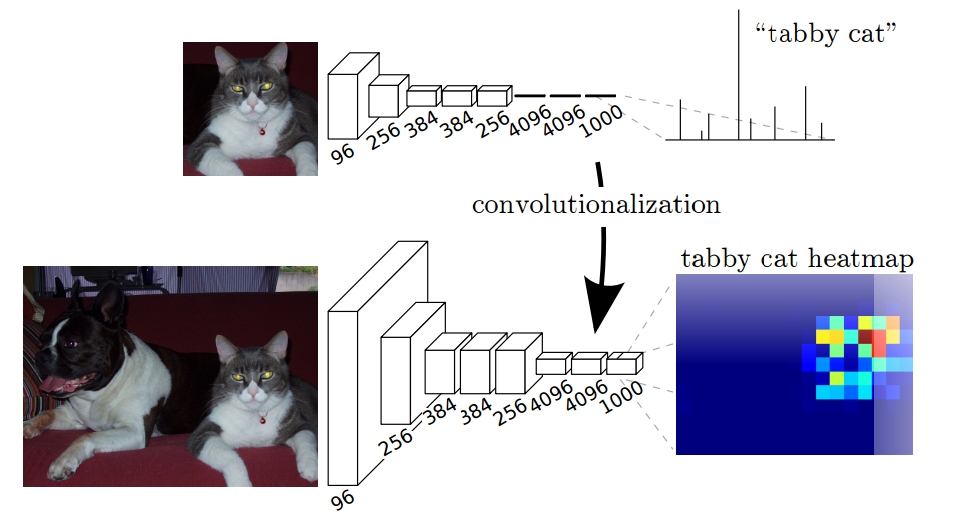
\includegraphics[width=9cm]{figures/fcnn}
    \caption{Comparison of a \gls{CNN} for classification (top) and a \gls{FCN} which creates a heat map (bottom). \cite{long2014fully}}
    \label{fig:fcn}
\end{figure}

\subsection{Fully connected convolutional layer}
A fully connected convolutional layer is a regular convolutional layer in size
of the input. Consequentially the weight matrix covers every input neuron. Long
noted in \cite{long2014fully} that it is the two dimensional equivalent to
fully connected layer in a classification \gls{CNN}.

\subsection{Deconvolutional Layer}
Deconvolutions are inverse convolutions. In context of neural networks the
function for forward and backward calculation are just switched. It is often combined with unpooling and allows to learn how to reconstruct a larger image region from a smaller input. Long indicate in \cite{long2014fully} its similarity to interpolation. He explains it as highly parametrized non-linear interpolation.
